%\textcolor{red}{Adaptive Mesh Refinement}

\chapter{AST Traversal}
%\chapter{AST Processing\{Traversal\}}
\label{AstProcessing:astProcessing}

\fixme{ This chapter should cover both the classic Object-Oriented Visitor Pattern
        Traversal (which has yet to be built, but which I understand Markus is prepared to
        implement) and the two new traversals based on iteration over the memory pools
        which Dan built in the latest internal release of ROSE in December 2005. 
        The three of these that are implemented are presenting in the ROSE Tutorial
        where there is a section for the unimplemented classic Object-Oriented Visitor Pattern
        Traversal not based on memory pools as a place holder (only the code need be updated).}

\section{Introduction}
\label{AstProcessing:introduction}
Tree traversal is a fundamental operation used to visit each node in a tree
data structure in a systematic way. Such traversals are categorized by the
order in which the nodes are visited. A traversal can start at the root and
explore as far as possible along each branch before backtracking, which is
referred to as a depth-first traversal. It can also be breadth-first
traversal\fixme{Does ROSE support breadth-first traversal?} which begins at the root node
and explores all nodes at depth level 1, then nodes at level 2, and so on. 
For depth-first traversal of a binary tree, it can in turn have three
variants: preorder (parent, left-child, right-child), inorder (left-child,
parent, right-child), or postorder (left-child, right-child, parent).
Inorder traversal does not make too much sense for tree nodes with varying
number of children since the "in" position of a parent among its children
is not well defined.  
Please note that postorder (left-child, right-child, parent) is
\textbf{NOT} equal to the reversed order of preorder (right-child, left-child, parent).  

ROSE aids the library writer by providing a traversal
mechanism that visits all the nodes of the AST in a predefined order
and to compute attributes.  Based on a fixed traversal order, we
provide inherited attributes for passing information down the AST (top-down processing) and synthesized attributes for passing information up
the AST (bottom-up processing). Inherited attributes can be used to
propagate context information along the edges of the AST, whereas
synthesized attributes can be used to compute values based on the
information of the subtree.  One function for computing inherited
attributes and one function for computing synthesized attributes must
be implemented when attributes are used.  We provide different
interfaces that allow both, one, or no attribute to be used; in
the latter case it is a simple traversal with a visit method called at
each node.

The AST processing mechanism can be used to gather information
about the AST, or to ``query'' the AST. Only the functions that are
invoked by the AST processing mechanism need to be implemented by the user
of AstProcessing classes; no traversal code must be implemented.

\section{Common Interface of the Processing Classes}

All five Ast*Processing classes provide three different functions for invoking a traversal on the AST:

\begin{description}
\item[T traverse(SgNode* node, ...):] traverse full AST (including nodes that represent code from include files)
\item[T traverseInputFiles(SgProject* projectNode, ...):] traverse the subtree of the AST
    that represents the file(s) specified on the command line to a translator; files that
    are the {\em input} to the translator.
\item[T traverseWithinFile(SgNode* node, ...):] traverse only those nodes that represent 
code of the same file where the traversal started. The traversal stays {\em within} the file.
\end{description}

The return type {\tt T} and the other parameters are discussed for each {\tt Ast*Processing} class in the following sections.

Further, the following virtual methods can be defined by the user (the default
implementations are empty):
\begin{description}
\item[void atTraversalStart():] called by the traversal code to signal to the
processing class that a traversal is about to start
\item[void atTraversalEnd():] called by the traversal code to signal that a
traversal has terminated (all nodes have been visited)
\end{description}

As these methods are the same for all processing classes, they are not
repeated in the class descriptions below.

\section{AstSimpleProcessing}
\label{AstProcessing:AstSimpleProcessing}

This class is called {\em Simple} because, in contrast to three of the other
processing classes, it does not provide the computation of
attributes. It implements a traversal of the AST and calls a
visit function at each node of the AST. This can be done as
a preorder or postorder traversal.

{\indent
%{\mySmallFontSize
{\footnotesize
\begin{verbatim}
     typedef {preorder,postorder} t_traversalOrder;

     class AstSimpleProcessing {
        public:
           void traverse(SgNode* node, t_traversalOrder treeTraversalOrder);
           void traverseWithinFile(SgNode* node, t_traversalOrder treeTraversalOrder);
           void traverseInputFiles(SgProject* projectNode, t_traversalOrder treeTraversalOrder);
        protected:
           void virtual visit(SgNode* astNode)=0;
     };
\end{verbatim}
}}
To use the class AstSimpleProcessing the user needs to implement the
function {\tt visit} for a user-defined class that inherits
from class AstSimpleProcessing. To invoke a traversal, one of the three
traverse functions needs to be called.

\subsection{Example}

In this example, we traverse the AST in preorder and print the name of
each node in the order in which they are visited.

The following steps are necessary:

\begin{description}
   \item[Interface:] Create a class, {\em MyVisitor}, that inherits from {\tt AstSimpleProcessing}.
   \item[Implementation:] Implement the function {\tt visit(SgNode* astNode)} for class {\em MyVisitor}.
   \item[Usage:] Create an object of type {\em MyVisitor} and invoke the function 
     {\tt traverse (SgNode* node, t\_traverseOrder treeTraversalOrder)}.
\end{description}

\begin{figure}
\begin{latexonly}
   \lstinputlisting{AstProcessing/MyVisitor.h}
\end{latexonly}

% Do this when processing latex to build html (using latex2html)
\begin{htmlonly}
   \verbatiminput{AstProcessing/MyVisitor.h}
\end{htmlonly}
\caption{Headerfile {\em MyVisitor.h}.}
\label{AstProcessing:myvisitor1}
\end{figure}

Figure \ref{AstProcessing:myvisitor1} presents the interface.

\begin{figure}
\begin{latexonly}
   \lstinputlisting{AstProcessing/MyVisitor.C}
\end{latexonly}

% Do this when processing latex to build html (using latex2html)
\begin{htmlonly}
   \verbatiminput{AstProcessing/MyVisitor.C}
\end{htmlonly}
\caption{Implementation file {\em MyVisitor.C}.}
\label{AstProcessing:myvisitor2}
\end{figure}

Figure \ref{AstProcessing:myvisitor2} presents the implementation.

\begin{figure}
\begin{latexonly}
   \lstinputlisting{AstProcessing/MyVisitorMain.C}
\end{latexonly}

% Do this when processing latex to build html (using latex2html)
\begin{htmlonly}
   \verbatiminput{AstProcessing/MyVisitorMain.C}
\end{htmlonly}
\caption{Example main program {\em MyVisitorMain.C}.}
\label{AstProcessing:myvisitor3}
\end{figure}

Figure \ref{AstProcessing:myvisitor3} presents the useage.

\section{AstPrePostProcessing}
\label{AstProcessing:AstPrePostProcessing}

The {\tt AstPrePostProcessing} class is another traversal class that does not
use attributes. In contrast to the {\tt AstSimpleProcessing} class, which
performs either a preorder or a postorder traversal, {\tt
AstPrePostProcessing} has both a preorder and a postorder component. Two
different visit methods must be implemented, one of which is invoked in
preorder (before the child nodes are visited), while the other is invoked in
postorder (after all child nodes have been visited). This traversal is
therefore well-suited for applications that require actions to be triggered
when `entering' or `leaving' certain subtrees of the AST.

{\indent
{\mySmallFontSize
\begin{verbatim}
     class AstPrePostProcessing {
        public:
           void traverse(SgNode* node);
           void traverseWithinFile(SgNode* node);
           void traverseInputFiles(SgProject* projectNode);
        protected:
           virtual void preOrderVisit(SgNode *node) = 0;
           virtual void postOrderVisit(SgNode *node) = 0;
     };
\end{verbatim}
}}

The user needs to implement the {\tt preOrderVisit} and {\tt postOrderVisit}
methods which are called before and after visiting child nodes, respectively.

\section{AstTopDownProcessing}
\label{AstProcessing:AstTopDownProcessing}

This class allows the user to use a restricted form of inherited attributes to
be computed for the AST. The user needs to implement the function
evaluateInheritedAttribute. This function is called for each node when
the AST is traversed. The inherited attributes are restricted such
that a single attribute of a parent node is inherited by all its child
nodes (i.e., the return value computed by the function {\tt evaluateInheritedValue} 
at the parent node is the input value to the function {\tt evaluateInheritedValue} 
at all child nodes).

{\indent
{\mySmallFontSize
\begin{verbatim}
     template<InheritedAttributeType>
     class AstTopDownProcessing {
        public:
           void traverse(SgNode* node, InheritedAttributeType initialInheritedAttribute);
           void traverseWithinFile(SgNode* node, InheritedAttributeType initialInheritedAttribute);
           void traverseInputFiles(SgProject* projectNode, InheritedAttributeType initialInheritedAttribute);
        protected:
           InheritedAttributeType 
           virtual evaluateInheritedAttribute(SgNode* astNode, InheritedAttributeType inheritedValue)=0;
           void virtual destroyInheritedValue(SgNode* astNode, InheritedAttributeType inheritedValue);
   };
\end{verbatim}
}}

The function {\tt evaluateInheritedAttribute} is called at each node. The traversal is a preorder traversal.

In certain rare cases, the inherited attribute computed at a node may involve
resources that must be freed; for instance, the attribute may be a pointer to
dynamically-allocated memory that is no longer needed after the traversal of
the child nodes has been completed. (Dynamically allocated attributes are only
recommended for very large attributes where copying would be prohibitively
expensive.) In such cases the {\tt destroyInheritedValue} method may be
implemented. This method is invoked with the inherited attribute computed at
this node after all child nodes have been visited. It can free any resources
necessary. An empty default implementation of this method is provided, so the
method can be ignored if it is not needed.

\subsection{Example}
   In this example, we traverse the AST and print the node names with proper indentation,
according to the nesting level of C++ basic blocks. The function 
{\tt evaluateInheritedAttribute} is implemented and an inherited attribute is used to
compute the nesting level.

The following steps are necessary:
\begin{description}
\item[Interface:] Create a class, {\em MyIndenting}, which inherits from AstTopDownProcessing, and a class {\tt MyIndentLevel}. The latter will be used for attributes. Note that the constructor of the class {\tt MyIndentLevel} initializes the attribute value.
\item[Implementation:] Implement the function {\tt evaluateInheritedAttribute(SgNode* astNode)} for class {\tt MyIndenting}.
\item[Usage:] Create an object of type {\em MyIndenting} and invoke the function traverse(SgNode* node, t\_traverseOrder treeTraversalOrder);
\end{description}

% Interface:
\begin{figure}
\begin{latexonly}
   \lstinputlisting{AstProcessing/MyIndenting.h}
\end{latexonly}

% Do this when processing latex to build html (using latex2html)
\begin{htmlonly}
   \verbatiminput{AstProcessing/MyIndenting.h}
\end{htmlonly}
\caption{Headerfile {\em MyIndenting.h}.}
\label{AstProcessing:myvisitor4}
\end{figure}

Figure \ref{AstProcessing:myvisitor4} presents the interface.

% Implementation:
\begin{figure}
\begin{latexonly}
   \lstinputlisting{AstProcessing/MyIndenting.C}
\end{latexonly}

% Do this when processing latex to build html (using latex2html)
\begin{htmlonly}
   \verbatiminput{AstProcessing/MyIndenting.C}
\end{htmlonly}
\caption{Implementation file {\em MyIndenting.C}.}
\label{AstProcessing:myvisitor5}
\end{figure}

Figure \ref{AstProcessing:myvisitor5} presents the implementation.

% Usage:
\begin{figure}
\begin{latexonly}
   \lstinputlisting{AstProcessing/MyVisitorMain.C}
\end{latexonly}

% Do this when processing latex to build html (using latex2html)
\begin{htmlonly}
   \verbatiminput{AstProcessing/MyIndentingMain.C}
\end{htmlonly}
\caption{Example main program {\em MyIndentingMain.C}.}
\label{AstProcessing:myvisitor6}
\end{figure}

Figure \ref{AstProcessing:myvisitor6} presents the useage.


Note that we could also use {\tt unsigned int} as attribute type in this 
simple example. But in general, the use of objects as attributes is more 
flexible and necessary, if you need to compute more than one attribute 
value (in the same traversal).

\section{AstBottomUpProcessing}
\label{AstProcessing:AstBottomUpProcessing}

This class allows to use synthesized attributes. The user needs to
implement the function evaluateSynthesizedAttribute to compute from a
list of synthesized attributes a single return value. Each element in the list is the
result computed at one of the child nodes in the AST. The return value is the synthesized
attribute value computed at this node and passed upwards in the AST.

{\indent
{\mySmallFontSize
\begin{verbatim}
     template<SynthesizedAttributeType>
     class AstBottomUpProcessing {
        public:
           SynthesizedAttributeType traverse(SgNode* node);
           SynthesizedAttributeType traverseWithinFile(SgNode* node);
           void traverseInputFiles(SgProject* projectNode);
           typedef ... SynthesizedAttributesList;
        protected:
           SynthesizedAttributeType
           virtual evaluateSynthesizedAttribute(SgNode* astNode, SynthesizedAttributesList synList)=0;
           SynthesizedAttributeType
           virtual defaultSynthesizedAttribute();
   };
\end{verbatim}
}}

   The type {\tt SynthesizedAttributesList} is an opaque typedef that in most
cases behaves like a Standard Template Library (STL) vector of objects of type
{\tt SynthesizedAttributeType}; in particular, it provides iterators and can
be indexed like a vector. The main difference to vectors is that no
operations for inserting or deleting elements or otherwise resizing the
container are provided. These should not be necessary as the list of
synthesized attributes is only meant to be read, not modified.

Using an iterator to operate on the list is necessary when the number of child nodes
is arbitrary. For example, in a SgBasicBlock, the number of {\tt SgStatement} nodes that are
child nodes ranges from 0 to {\tt n}, where {\tt n = synList.size()}.
For AST nodes with a fixed number of child nodes these values can be accessed by name,
using enums defined for each AST node class. The naming scheme for attribute access is
{\tt <CLASSNAME>\_<MEMBERVARIABLENAME>}.

   The method {\tt defaultSynthesizedAttribute} must be used to initialize attributes of
primitive type (such as int, bool, etc.).  This method is called when a synthesized
attribute needs to be created for a non-existing subtree  (i.e. when a node-pointer is
null). A null pointer is never passed to an evaluate function. If a class is used to
represent a synthesized attribute, this method does not need to be implemented because
the default constructor is called. In order to define an default value for attributes
of primitive type, this method must be used.

   Two cases exist when a default value is used for a synthesized attribute
and the defaultSynthesizedAttribute method is called:
\begin{itemize}
\item When the traversal encounters a null-pointer it will not call an evaluate method but
      instead calls defaultSynthesizedAttribute.
\item When the traversal skips over specific IR nodes. For example, 
      {\tt traverseInputFiles()} only calls the evaluate method on nodes which represent
      the input-file(s) but skips all other nodes (of header files for example).
\end{itemize}

% \subsection{Example: Node pointers as synthesized attribute values}
%In this example we show how to make all node pointers accessible as synthesized attributes.
%TODO

\subsection{Example: Access of Synthesized Attribute by Name}

The enum definition used to access the synthesized attributes by name at 
a {\tt SgForStatement} node is:
{\indent
{\mySmallFontSize
\begin{verbatim}
     enum E_SgForStatement {SgForStatement_init_stmt, SgForStatement_test_expr_root, SgForStatement_increment_expr_root, SgForStatement_loop_body};
\end{verbatim}
}}
The definitions of the enums for all AST nodes can be found in the generated file
\verb+<COMPILETREE>/SAGE/Cxx_GrammarTreeTraversalAccessEnums.h+.

For example, to access the synthesized attribute value of the SgForStatement's
test-expression the synthesized attributes list is accessed using the enum definition
for the test-expr. In the example we assign the pointer to a child node to a variable
{\tt myTestExprSynValue}:

{\indent
{\mySmallFontSize
\begin{verbatim}
SgNode* myTestExprSynValue=synList[SgForStatement_test_expr_root].node;
\end{verbatim}
}}
For each node with a fixed number of child nodes, the size of the synthesized
attributes value list is always the same size, independent of whether the children
exist or not. For example, for the SgForStatement it is always of size 4. If a child
does not exist, the synthesized attribute value is the default value of the respective
type used for the synthesized attribute (as template parameter).

\section{AstTopDownBottomUpProcessing}
\label{AstProcessing:AstTopDownBottomUpProcessing}

This class combines all features from the two classes that were previously presented.  It
allows the user to use inherited and synthesized attributes. Therefore, the user needs
to provide an implementation for two virtual functions, for
evaluateInheritedAttribute and evaluateSynthesizedAttribute. The
signature for evaluateSynthesizedAttribute has an inherited attribute
as an additional parameter. This allows the results of
inherited and synthesized attributes to be combined. You can use the
inherited attribute that is computed at a
node A by the evaluateInheritedAttribute method in the evaluateSynthesizedAttribute method at node A. But you cannot
use synthesized attributes for computing inherited attributes (which is obvious from the method signatures). If such a data
dependence needs to be represented, member variables of the traversal
object can be used to {\em simulate} such a behavior to some
degree. Essentially, this allows for the implementation of a pattern, also called
{\em accumulation.} For example, building a list of all nodes of the AST
can be implemented using this technique.

{\indent
{\footnotesize
\begin{verbatim}
     template<InheritedAttributeType, SynthesizedAttributeType>
     class AstTopDownBottomUpProcessing {
        public:
           SynthesizedAttributeType traverse(SgNode* node, 
                 InheritedAttributeType initialInheritedAttribute);

           SynthesizedAttributeType traverseWithinFile(SgNode* node, 
                 InheritedAttributeType initialInheritedAttribute);

           void traverseInputFiles(SgProject* projectNode, 
                 InheritedAttributeType initialInheritedAttribute);

           typedef ... SynthesizedAttributesList;
        protected:
           InheritedAttributeType
           virtual evaluateInheritedAttribute(SgNode* astNode, InheritedAttributeType inheritedValue);
           SynthesizedAttributeType
           virtual evaluateSynthesizedAttribute(SgNode* astNode, InheritedAttributeType inh, 
                            SynthesizedAttributesList synList)=0;
           SynthesizedAttributeType
           virtual defaultSynthesizedAttribute();
     };
\end{verbatim}
}
}

\section{Combined Processing Classes}

Running many read-only traversals on a single unchanged AST is an inefficient
operation because every node is visited many times. ROSE therefore provides
{\em combined} traversals that make it possible to run several traversals of
the same base type in a single traversal, reducing the overhead considerably.
Processing classes need not be adapted for use with the combined processing
framework, so existing traversals can be reused; new traversals can be
developed and tested independently and combined at any time.

To make sure that combined traversals work correctly, they should not change
the AST or any other shared data. Terminal output from combined processing
classes will be interleaved. No assumptions should be make about the order in
which the individual traversals will be executed on any node.

For each {\tt Ast*Processing} class there is a corresponding {\tt
AstCombined*Processing} class that behaves similarly. The interfaces for two
of these classes are presented below, the others are analogous.

{\indent
{\mySmallFontSize
\begin{verbatim}
     typedef {preorder,postorder} t_traversalOrder;

     class AstCombinedSimpleProcessing {
        public:
           void traverse(SgNode* node, t_traversalOrder treeTraversalOrder);
           void traverseWithinFile(SgNode* node, t_traversalOrder treeTraversalOrder);
           void traverseInputFiles(SgProject* projectNode, t_traversalOrder treeTraversalOrder);

           void addTraversal(AstSimpleProcessing* traversal);
           vector<AstSimpleProcessing*>& get_traversalPtrListRef();
     };
\end{verbatim}
}}

{\indent
{\mySmallFontSize
\begin{verbatim}
     template<InheritedAttributeType, SynthesizedAttributeType>
     class AstCombinedTopDownBottomUpProcessing {
        public:
           vector<SynthesizedAttributeType> 
             traverse(SgNode* node, vector<InheritedAttributeType> initialInheritedAttributes);
          
           vector<SynthesizedAttributeType> 
              traverseWithinFile(SgNode* node, vector<InheritedAttributeType> initialInheritedAttributes);
          
          void traverseInputFiles(SgProject* projectNode, vector<InheritedAttributeType> initialInheritedAttributes);
          
          typedef ... SynthesizedAttributesList;

           void addTraversal(AstTopDownBottomUpProcessing<InheritedAttributeType, SynthesizedAttributeType>* traversal);
           vector<AstTopDownBottomUpProcessing<InheritedAttributeType, SynthesizedAttributeType>*>
             & get_traversalPtrListRef();
     };
\end{verbatim}
}}

Note that these classes do not contain virtual functions for the user to
override. They are meant to be used through explicit instances, not as base
classes. Instead of calling one of the traverse methods on the individual
processing classes, they are combined within an instance of the {\tt
AstCombined*Processing} class and started collectively using one of its
traverse methods. Inherited and synthesized attributes are passed in and back
through STL vectors.

Two methods for managing the list of traversals are provided: The {\tt
addTraversal} method simply adds the given traversal to its list, while {\tt
get\_traversalPtrListRef} returns a reference to its internal list that allows
any other operations such as insertion using iterators, deletion of elements,
etc.

%\section{Traversal Order And Attribute Access}
%\label{AstProcessing:TraversalOrderAndAttributeAccess}
%TODO: generate a latex version using tables, a text version, and a dot
%version (without inheritance), and the inheritance graph
%(=doxygenoutput)

\section{AST Node Attributes}

To each node in the AST user-defined attributes can have an attribute attached to 
it {\em by name} (by defining a unique name, string, for the attribute). The
user needs to implement a class that inherits from {\tt AstAttribute}. Instances of this
class can be attached to an AST node by using member functions of {\tt SgNode::attribute}.

Example: let node be a pointer to an object of type SgNode:
{\indent
{\mySmallFontSize
\begin{verbatim}
     class MyAstAttribute : public AstAttribute {
        public:
	        MyAstAttribute(int v):value(v) {}
                virtual AstAttribute* copy() const override {
                    return new MyAstAttribute(*this);
                }
                virtual std::string attribute_class_name() const override {
                    return "MyAstAttribute";
                }
           ...
        private:
           int value;
           ...
     };

     node->attribute.setAttribute("mynewattribute",new MyAstAttribute(5));
\end{verbatim}
}}
Using this expression, an attribute with name {\tt mynewattribute} can
be attached to the AST node pointed to by node. Similarly, the same attribute can be
accessed {\em by name} using the member function getAttribute:

{\indent
{\mySmallFontSize
\begin{verbatim}
     MyAstAttribute* myattribute=node->attribute.getAttribute("mynewattribute");
\end{verbatim}
}}
AST attributes can be used to combine the results of different
processing phases. Different traversals that are performed in
sequence can store and read results to and from each node of the
AST. For example, the first traversal may attach its results for each node as
attributes to the AST, and the second traversal can read and use these results.


%===========================================================================
\section{Visualization}

\subsection{Example Graphs}

% Do this when processing latex to generate non-html (not using latex2html)
\begin{figure}
\begin{latexonly}
   \lstinputlisting{AstProcessing/astprocessingdoc_example1.C}
\end{latexonly}

% Do this when processing latex to build html (using latex2html)
\begin{htmlonly}
   \verbatiminput{AstProcessing/astprocessingdoc_example1.C}
\end{htmlonly}
\caption{Example program used as running example}
\label{AstProcessing:example1}
\end{figure}

\begin{figure}
%\centerline{\psfig{file=AstProcessing/astprocessingdoc_example1.Preorder.ps,height=1.0\linewidth,width=1.0\linewidth,angle=0}}
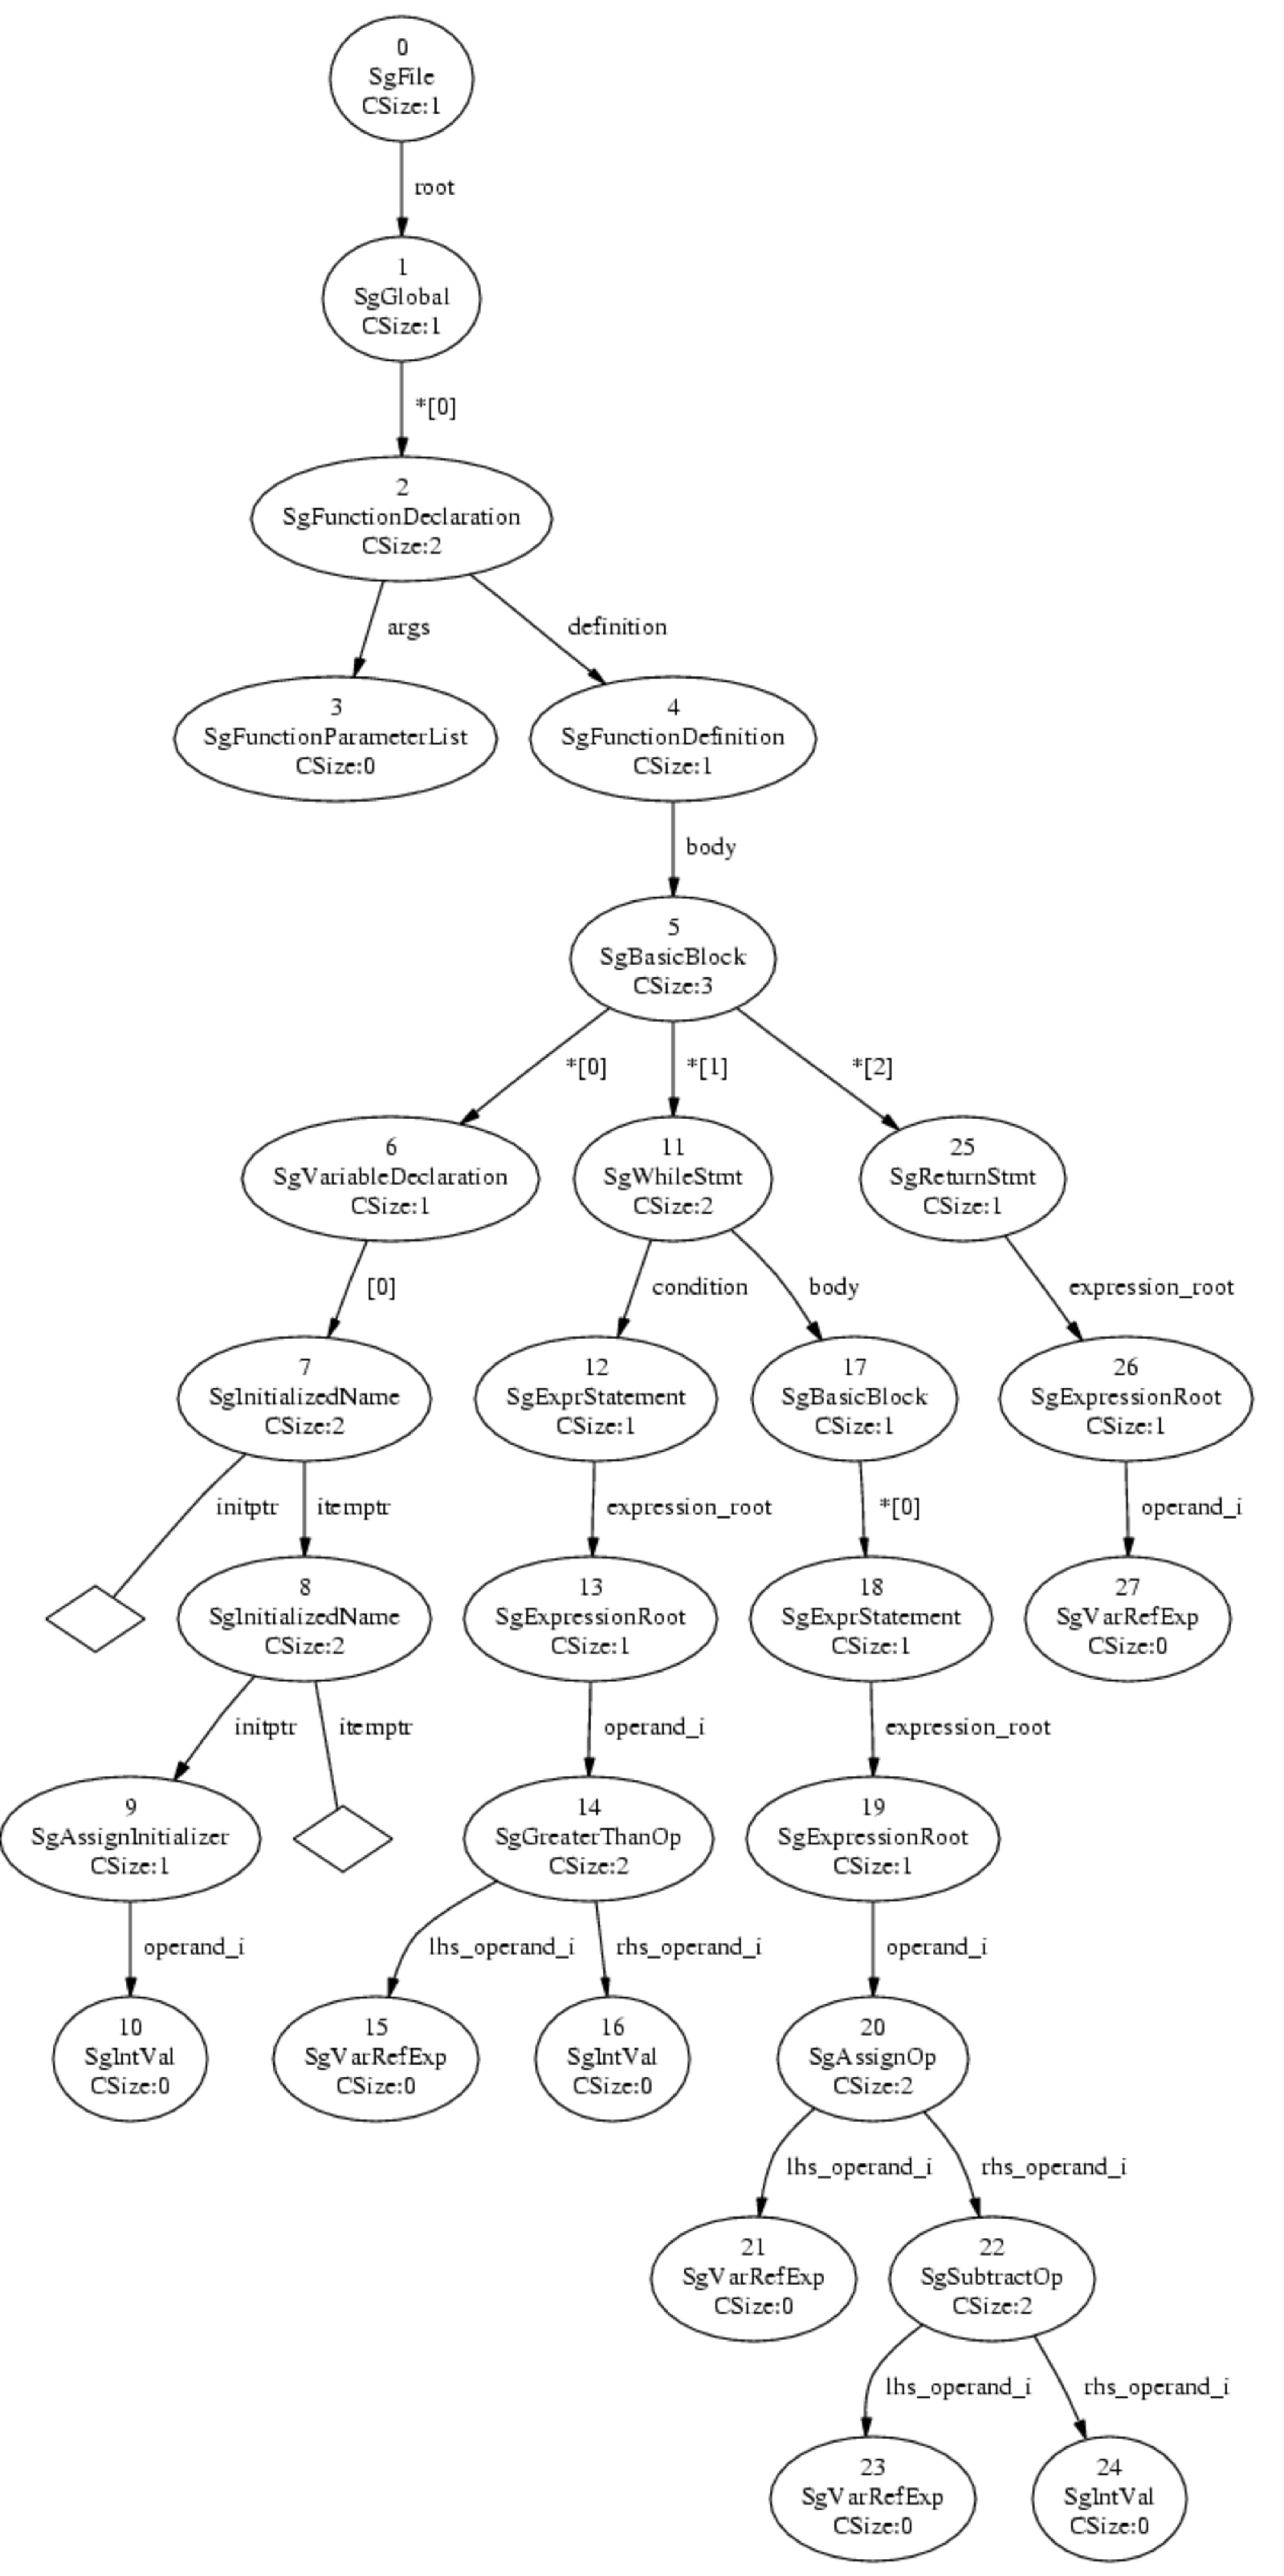
\includegraphics[scale=0.15]{AstProcessing/astprocessingdoc_example1_Preorder}
\caption{Numbers at nodes show the order in which the visit function is called in a preorder traversal}
\label{AstProcessing:PreorderAst}
\end{figure}

\begin{figure}
%\centerline{\psfig{file=AstProcessing/astprocessingdoc_example1.Postorder.ps,height=1.0\linewidth,width=1.0\linewidth,angle=0}}
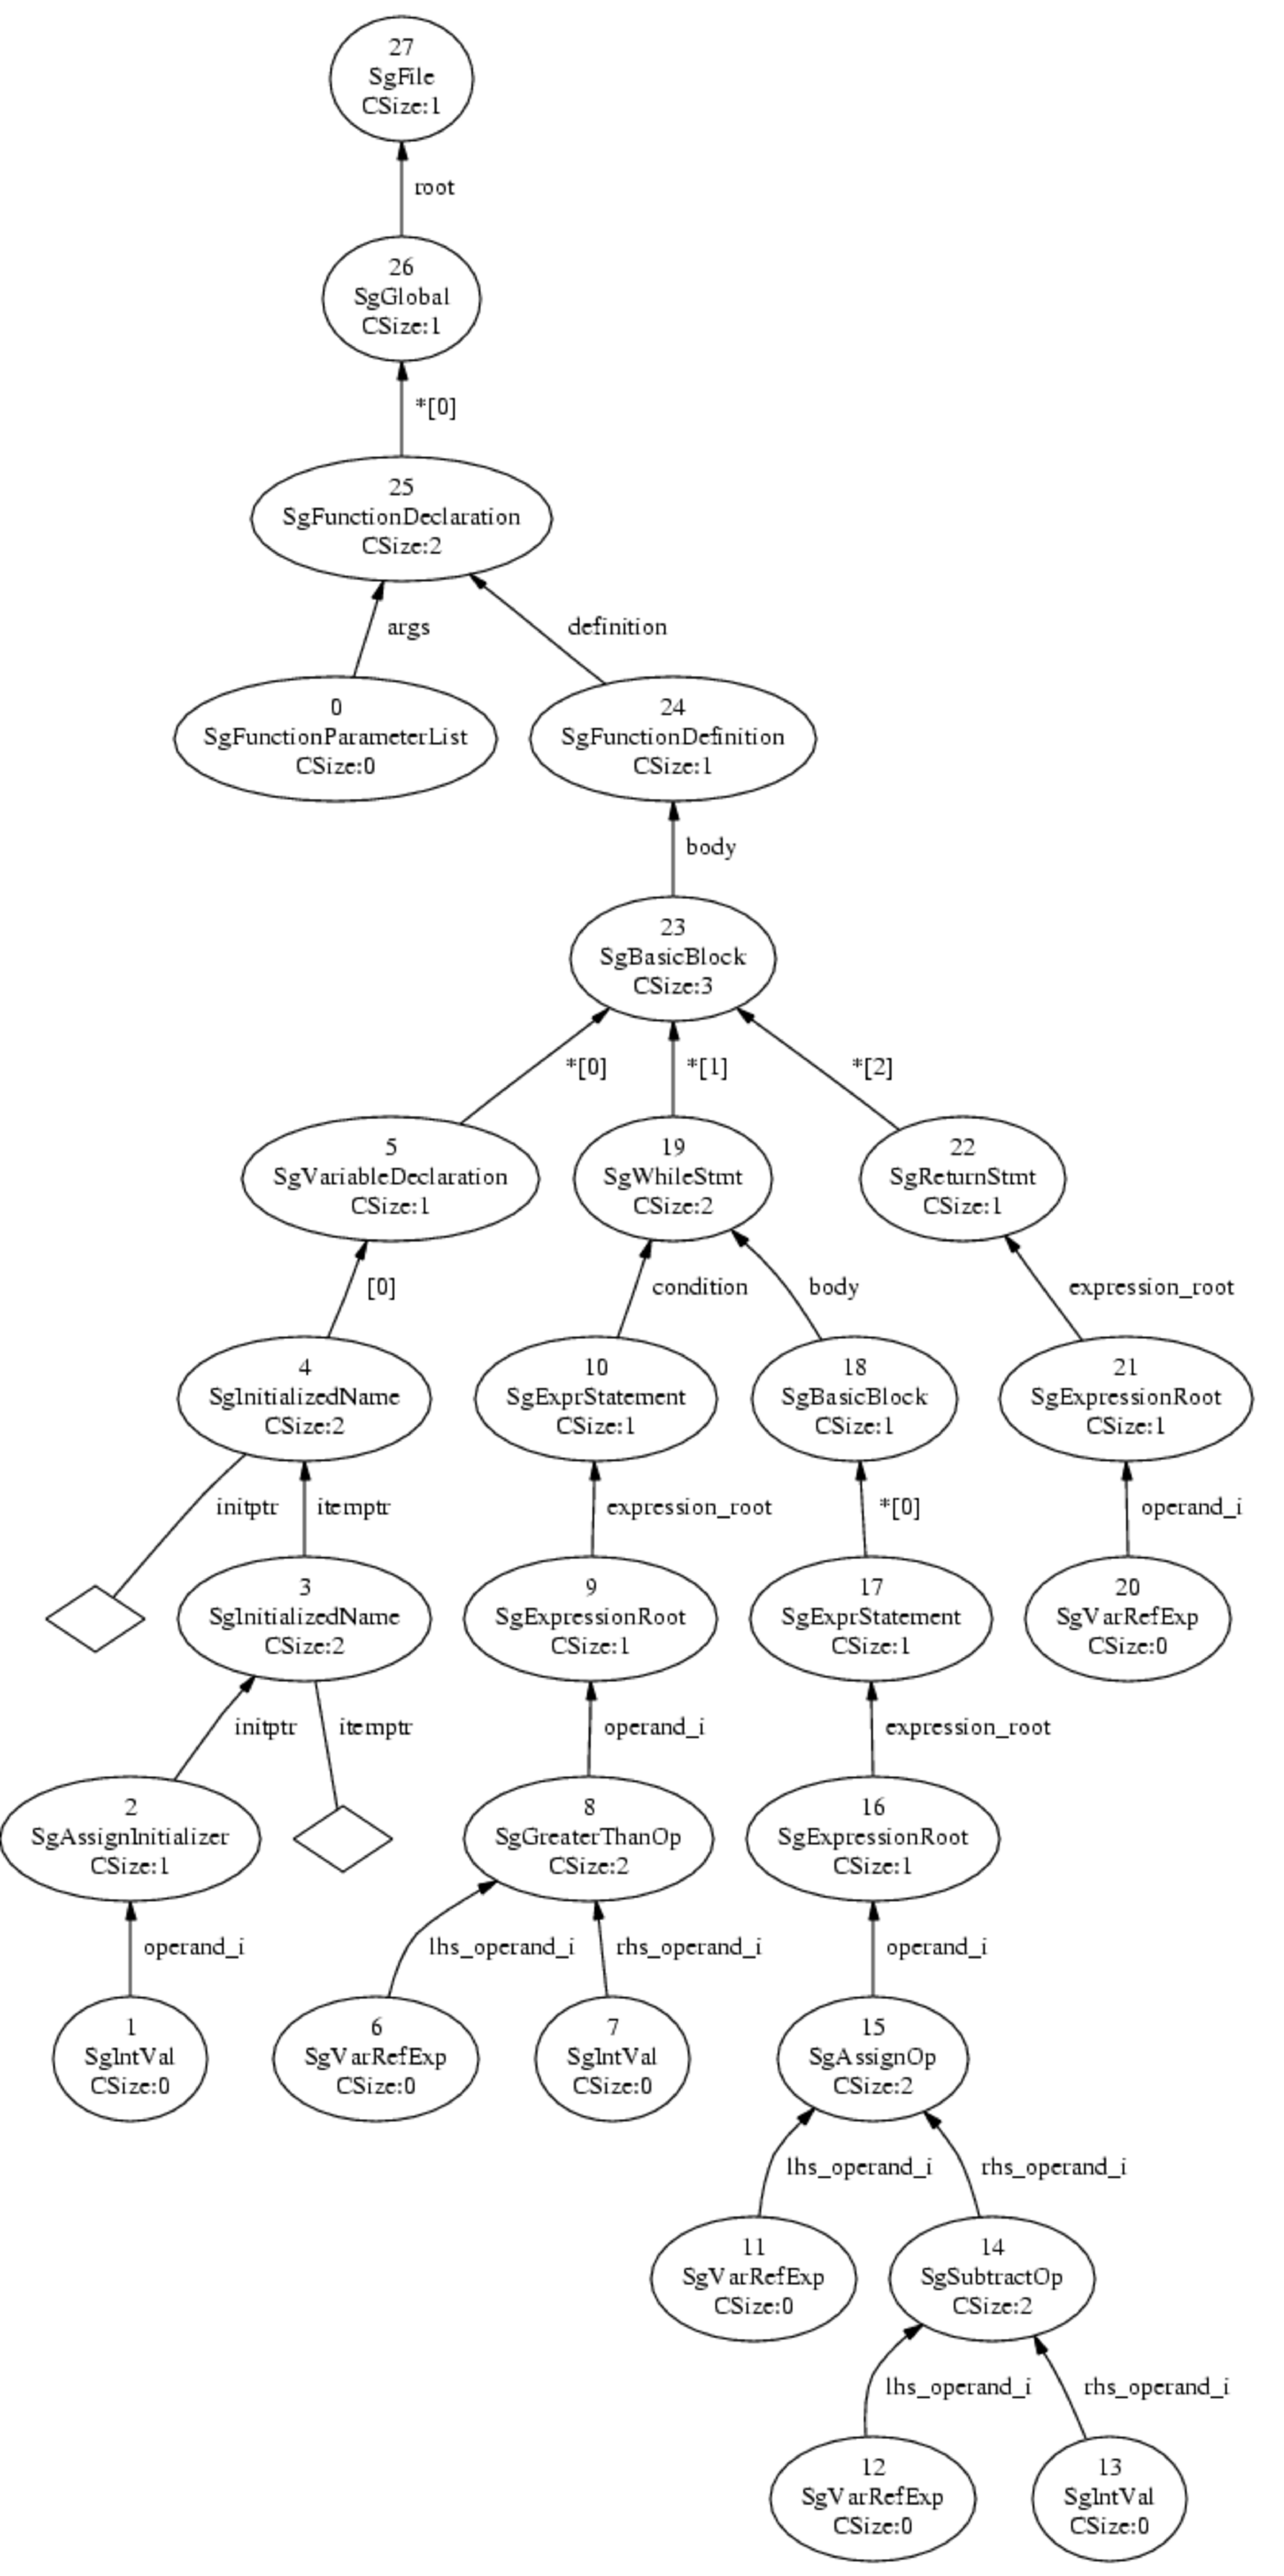
\includegraphics[scale=0.15]{AstProcessing/astprocessingdoc_example1_Postorder}
\caption{Numbers at nodes show the order in which the visit function is called in a postorder traversal}
\label{introduction:PostorderAst}
\end{figure}

The graph shown in figure \ref{AstProcessing:PreorderAst} is the AST of
the program in figure \ref{AstProcessing:example1}. Such an output can
be generated for an AST with:

{\indent
{\mySmallFontSize
\begin{verbatim}
     AstDOTGeneration dotgen;
     dotgen.generateInputFiles(projectNode, AstDOTGeneration::PREORDER);
\end{verbatim}
}}
where {\tt projectNode} is a node of type {\tt SgProjectNode} and the
order in which the AST is traversed is specified to be {\tt
AstDOTGeneration::PREORDER} (or {\tt AstDOTGeneration::POSTORDER}).

\begin{figure}
%\centerline{\psfig{file=AstProcessing/astprocessingdoc_example1.TopDown.ps,height=1.0\linewidth,width=1.0\linewidth,angle=0}}
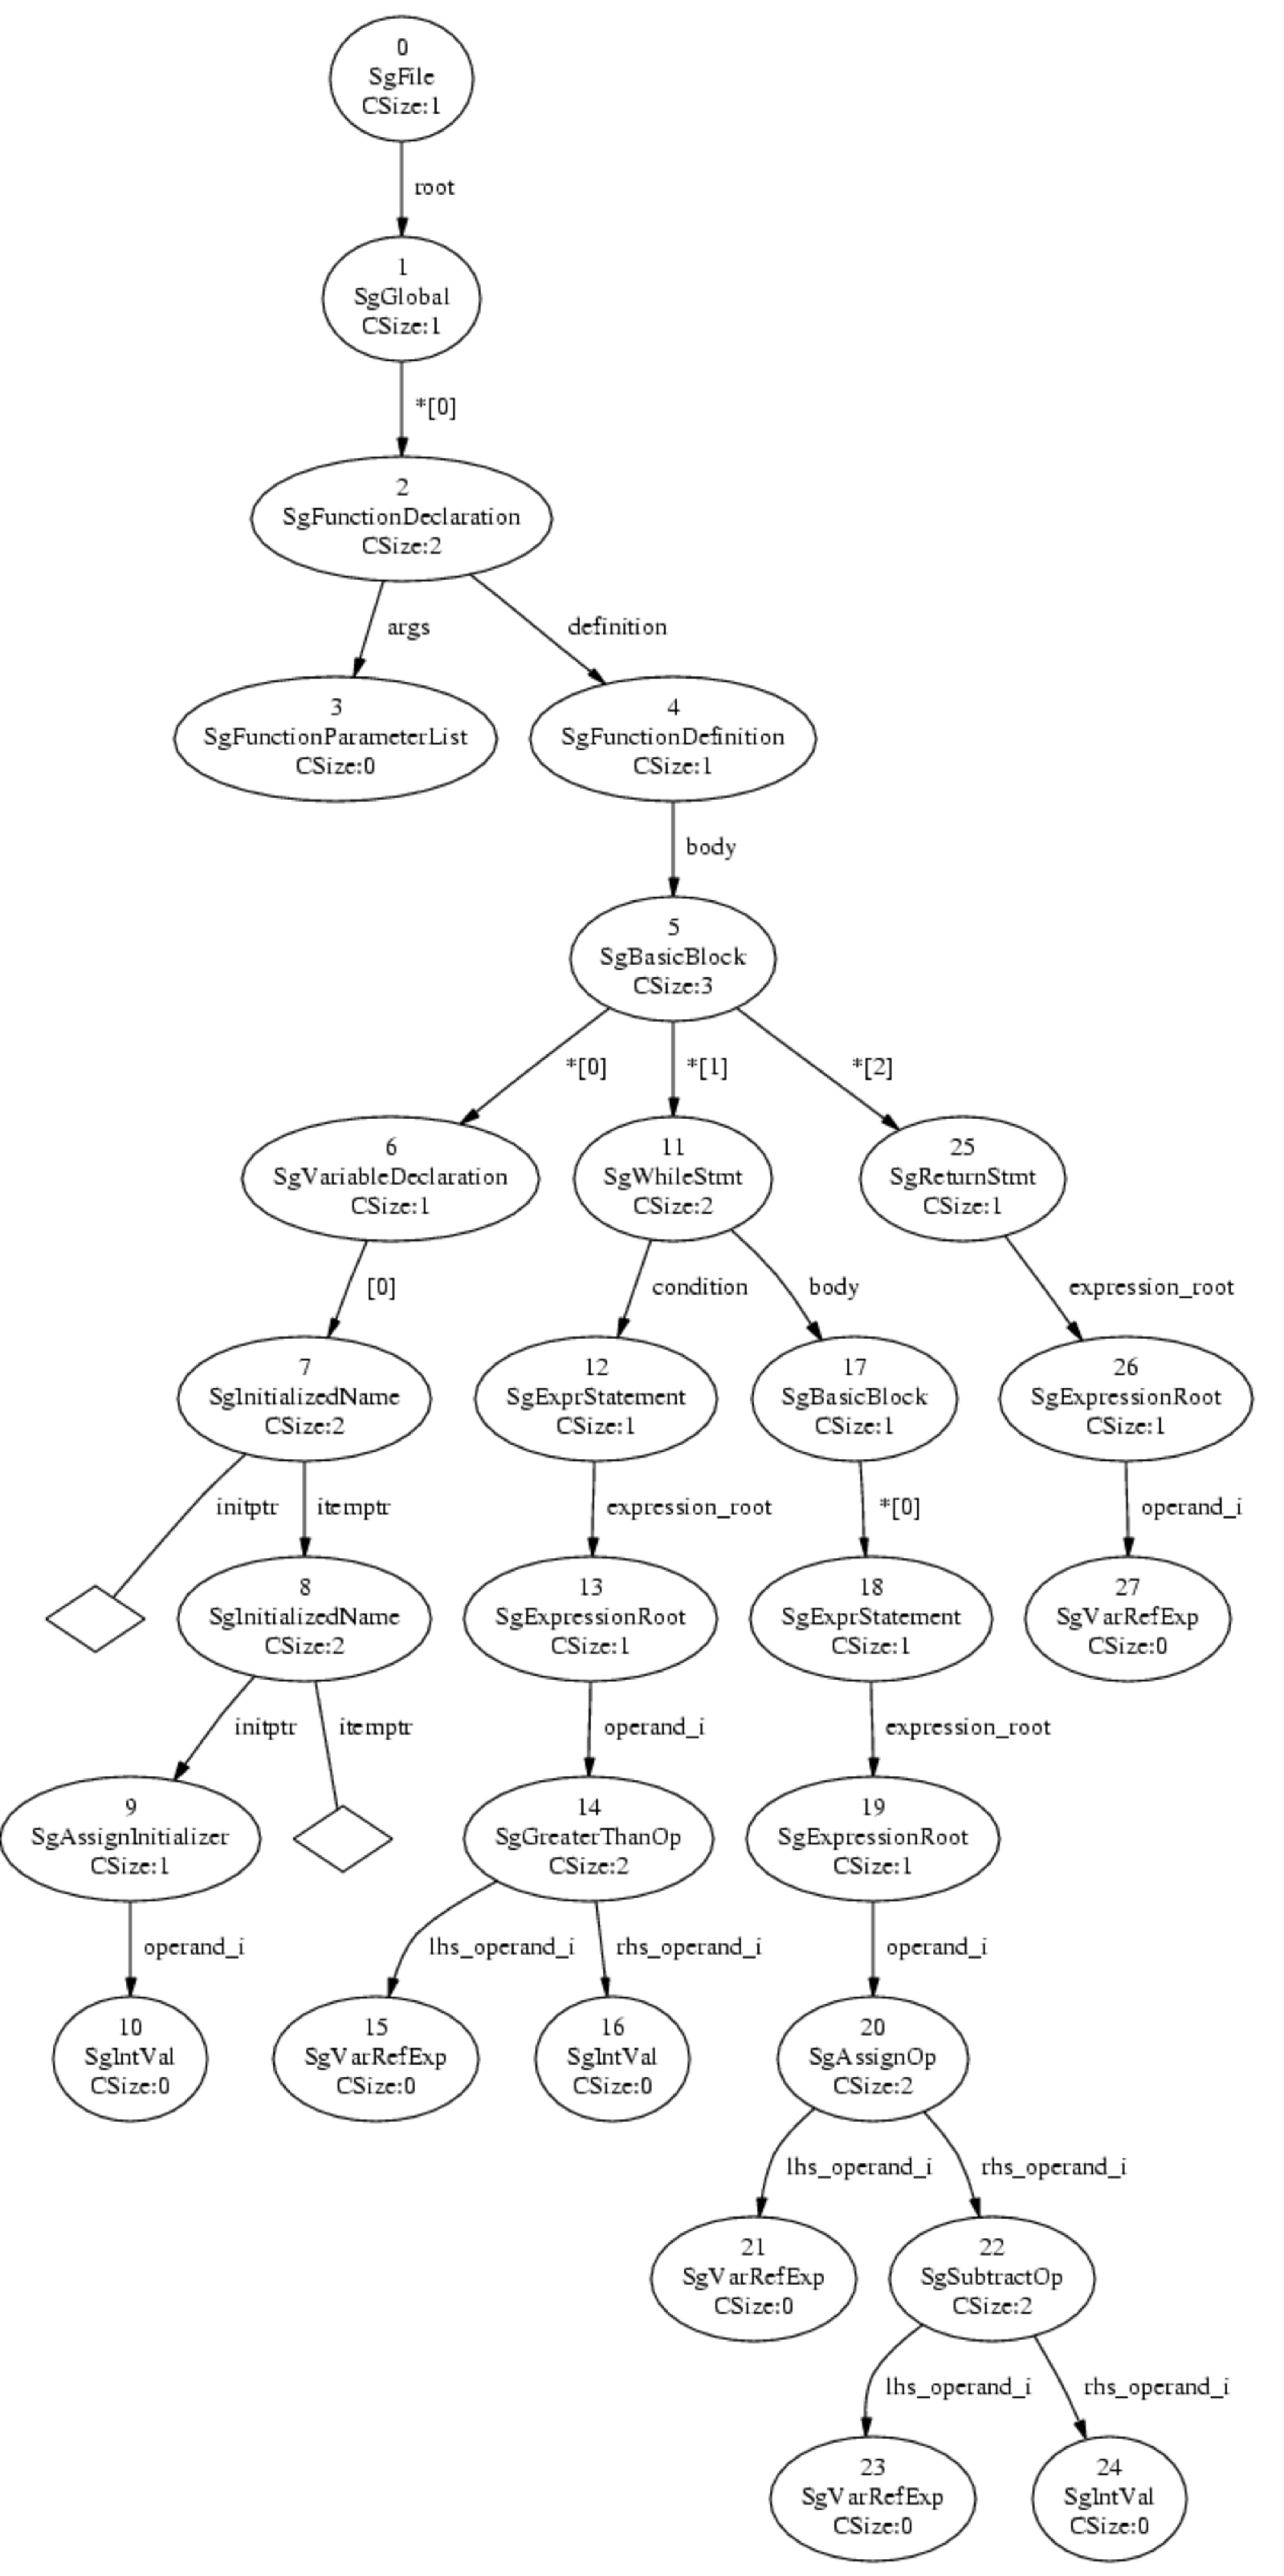
\includegraphics[scale=0.15]{AstProcessing/astprocessingdoc_example1_TopDown}
\caption{Numbers at nodes show the order in which the function evaluateInheritedAttribute is called in a top-down processing}
\label{AstProcessing:TopDownAst}
\end{figure}

\begin{figure}
%\centerline{\psfig{file=AstProcessing/astprocessingdoc_example1.BottomUp.ps,height=1.0\linewidth,width=1.0\linewidth,angle=0}}
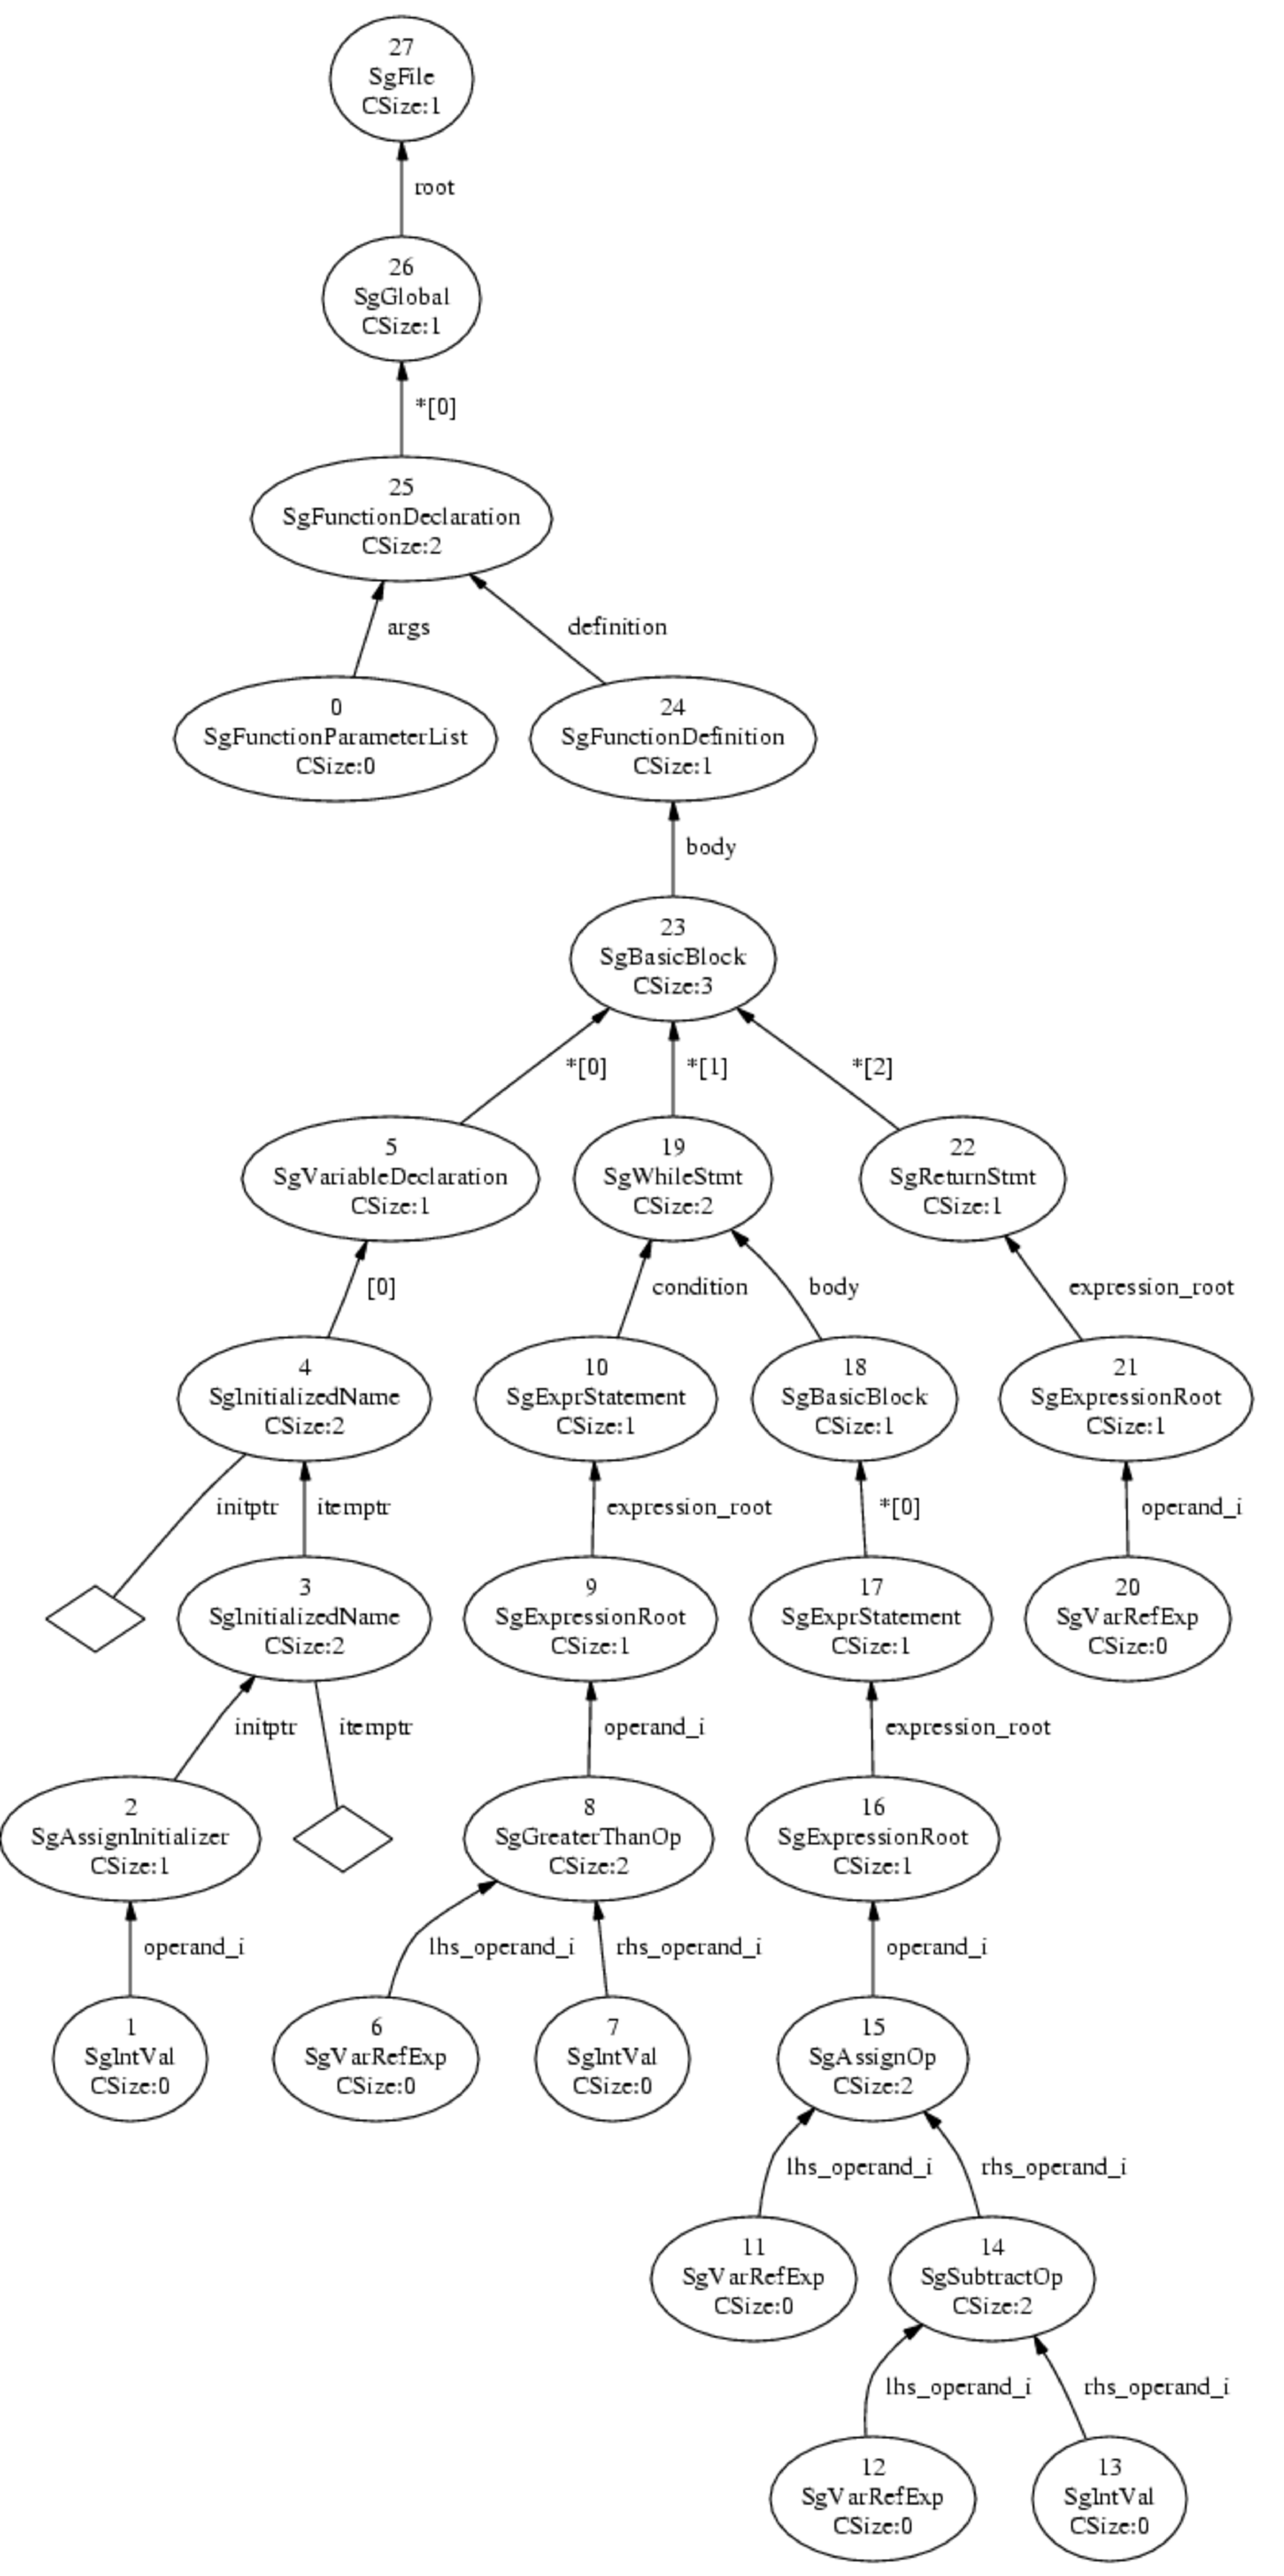
\includegraphics[scale=0.15]{AstProcessing/astprocessingdoc_example1_BottomUp}
\caption{Numbers at nodes show the order in which the function evaluateSynthesizedAttribute is called in a bottom up processing}
\label{AstProcessing:BottomUpAst}
\end{figure}

\begin{figure}
%\centerline{\psfig{file=AstProcessing/astprocessingdoc_example1.TopDownBottomUp.ps,height=1.0\linewidth,width=1.0\linewidth,angle=0}}
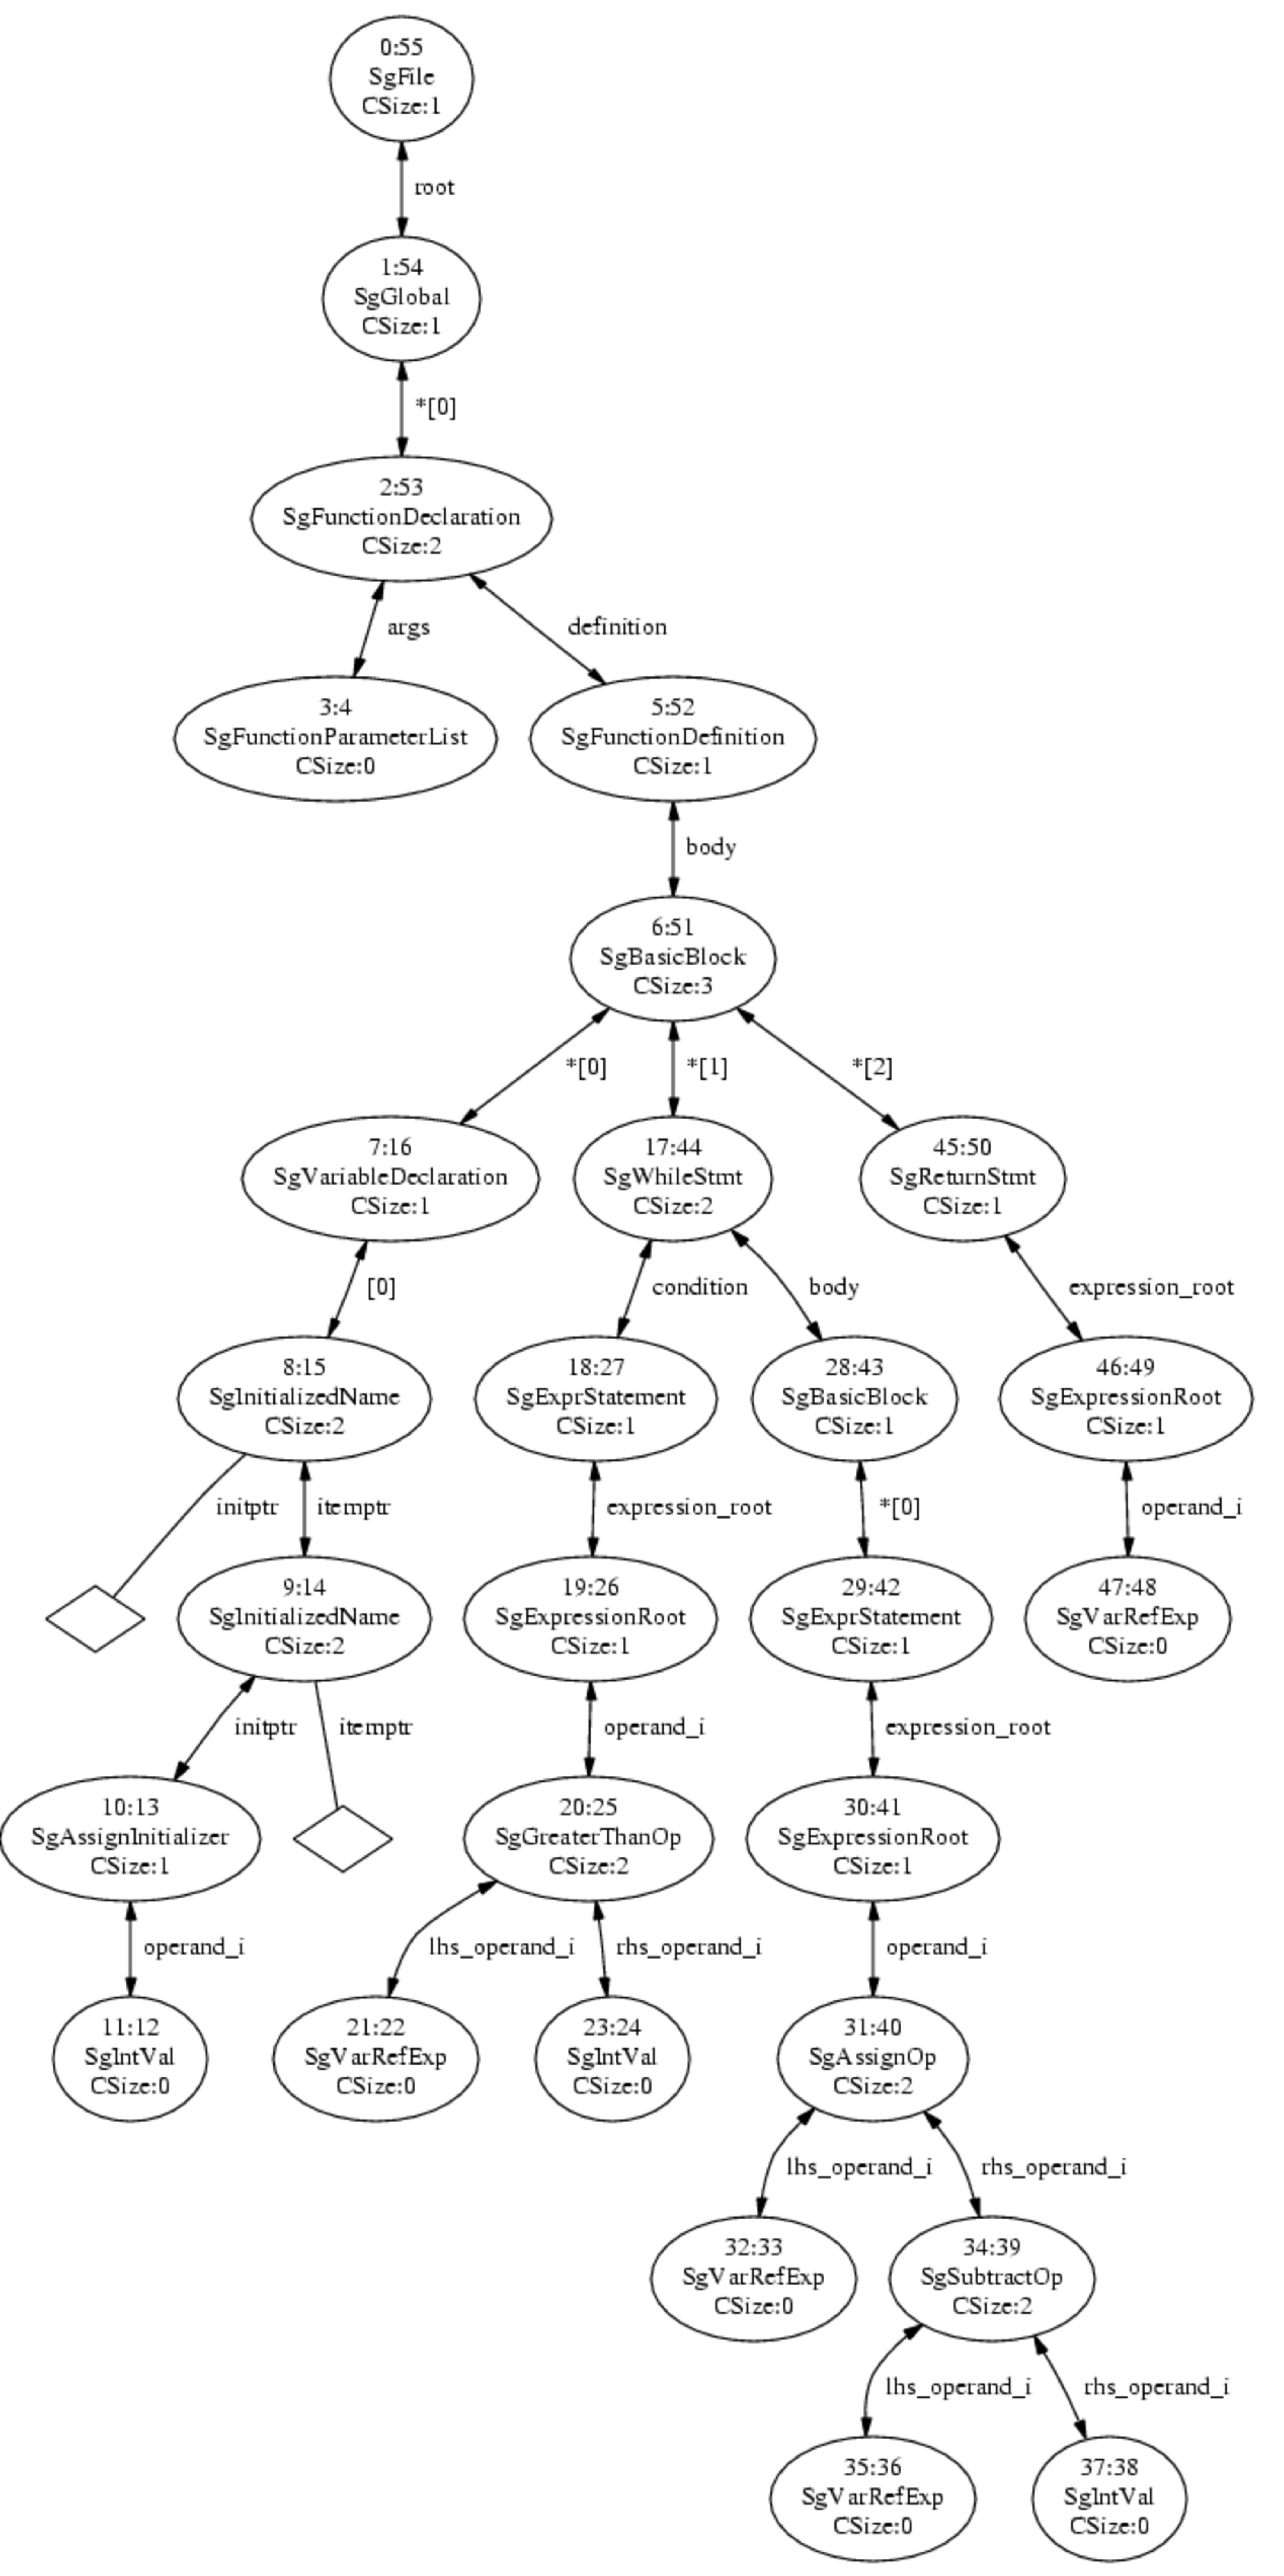
\includegraphics[scale=0.15]{AstProcessing/astprocessingdoc_example1_TopDownBottomUp}
\caption{The pair of numbers at nodes shows the order in which the function
    evaluateInheritedAttribute (first number) and evaluateSynthesizedAttribute (second number)
    is called in a top-down-bottom-up processing.}
\label{AstProcessing:TopDownBottomUpAst}
\end{figure}
%===========================================================================
\section{Conclusions}

All AST*Processing classes provide similar interfaces that differ only by the attributes used. AST node attributes can be used to attach data to each AST node and to share information between different traversals. 

Additional examples for traversal, attributes, pdf, and dot output can be found in 
\begin{itemize}
\item \verb+ROSE/exampleTranslators/documentedExamples/astProcessingExamples+.
\end{itemize}

Table~\ref{tab:sumTraversal} summaries and compares the traversal and query support in ROSE. 
It shows the types of SgNode visited, context, performance, order of nodes being visited, source files being visited, 
and suggested use for each of the choices. 
% Liao 4/21/2010 add a table to summary traversal/query
\begin{table}[htbp]
  \centering
\resizebox{7.0in}{!}{ % width of the table
\begin{tabular}{||l|c|p{1.0in}|c|p{0.8in}|c|p{1.0in}||} \hline

 \multicolumn{7}{||c||}{\textbf{\textcolor{blue}{Regular AST Traversal}}} \\\hline \hline
& \textbf{Node Types} & \textbf{Context} & \textbf{Performance} & \textbf{Order} & \textbf{File Visited} & \textbf{Suggested Use} \\ \hline
%ROSE\_VisitorPattern&  predefined & No & regular & configurable & configuration & Simple traversal \\ \hline
AstSimpleProcessing  &  & No & & pre or post order & & simple analysis \\ \cline{1-1}
\cline{3-3} \cline{5-5} \cline{7-7}
AstTopDownProcessing  & & attributes from parent nodes& & preorder & & inherited attributes \\  \cline{1-1}
\cline{3-3} \cline{5-5} \cline{7-7}
AstBottomUpProcessing & a predefined & attributes from child nodes & regular
& postorder & configurable & synthesized attribute \\  \cline{1-1}
\cline{3-3} \cline{5-5} \cline{7-7}
AstTopDownBottomUpProcessing & subset & attributes from both parent
and children & & pre and post order & & mixed inherited and synthesized
attributes \\ \cline{1-1}
\cline{3-3} \cline{5-5} \cline{7-7}
AstPrePostProcessing &  & No & & pre and post order & & mixed topdown and bottomup w/o attributes \\ \hline

 \multicolumn{7}{||c||}{\textbf{\textcolor{blue}{Combined AST Traversal}}} \\\hline \hline
%AstCombinedSimpleProcessing&  & & &  & & \\ \hline
AstCombinedSimpleProcessing &  \multicolumn{6}{|c||}{} \\ \cline{1-1}
AstCombinedTopDownProcessing &  \multicolumn{6}{|c||}{} \\ \cline{1-1}
AstcombinedBottomUpProcessing&  \multicolumn{6}{|c||}{Similar to the
corresponding traversals above but fuse multiple traversals into one} \\ \cline{1-1}
AstCombinedTopDownBottomUpProcessing & \multicolumn{6}{|c||}{} \\ \cline{1-1} 
AstCombinedPrePostProcessing& \multicolumn{6}{|c||}{} \\ \hline \hline

 \multicolumn{7}{||c||}{\textbf{\textcolor{blue}{Reverse AST Traversal}}} \\\hline \hline
AstReversePrefixSimpleProcessing &  \multicolumn{6}{|c||}{} \\ \cline{1-1}
AstReversePrefixInhProcessing &  \multicolumn{6}{|c||}{ ???? } \\ \cline{1-1}
AstReversePrefixSynProcessing &  \multicolumn{6}{|c||}{} \\ \cline{1-1}
AstReversePrefixInhSynProcessing &  \multicolumn{6}{|c||}{} \\ \hline \hline

AstReverseBranchSimpleProcessing &  \multicolumn{6}{|c||}{} \\ \cline{1-1}
AstReverseBranchInhProcessing &  \multicolumn{6}{|c||}{ ??? } \\ \cline{1-1}
AstReverseBranchSynProcessing &  \multicolumn{6}{|c||}{} \\ \cline{1-1}
AstReverseBranchInhSynProcessing &  \multicolumn{6}{|c||}{} \\ \hline \hline

 \multicolumn{7}{||c||}{\textbf{\textcolor{blue}{Parallel Traversal}}} \\\hline \hline
%& \textbf{Node Type Visited} & \textbf{Context} & \textbf{Performance} & \textbf{Order} & \textbf{File Visited} & \textbf{Suggested Use} \\ \hline
AstSharedMemoryParallelSimpleProcessing &  \multicolumn{6}{|c||}{} \\
\cline{1-1}
AstSharedMemoryParallelTopDownProcessing &  \multicolumn{6}{|c||}{} \\
\cline{1-1}
AstSharedMemoryParallelBottomUpProcessing &  \multicolumn{6}{|c||}{ Similar
to AstCombined*Processing if traverse() is called,} \\
\cline{1-1}
AstSharedMemoryParallelTopDownBottomUpProcessing &  \multicolumn{6}{|c||}{
but do parallel traversal via Pthreads if traverseInParallel() is called.}
\\ \cline{1-1}
AstSharedMemoryParallelPrePostProcessing &  \multicolumn{6}{|c||}{} \\
\hline \hline

AstSharedMemoryParallelizableSimpleProcessing &   \multicolumn{6}{|c||}{}
\\ \cline{1-1}
AstSharedMemoryParallelizableTopDownProcessing &  \multicolumn{6}{|c||}{}
\\ \cline{1-1} 
AstSharedMemoryParallelizableBottomUpProcessing &
\multicolumn{6}{|c||}{Internal use only, representing a traversal that}
\\ \cline{1-1}
AstSharedMemoryParallelizableTopDownBottomUpProcessing &
\multicolumn{6}{|c||}{ that can run in parallel without interfering others.} \\ \cline{1-1}
AstSharedMemoryParallelizablePrePostProcessing &  \multicolumn{6}{|c||}{}
\\ \hline \hline


 \multicolumn{7}{||c||}{\textbf{\textcolor{blue}{Memory Pool Traversal}}} \\\hline \hline
%& \textbf{Node Type Visited} & \textbf{Context} & \textbf{Performance} & \textbf{Order} & \textbf{File Visited} & \textbf{Suggested Use} \\ \hline
ROSE\_VisitTraversal & all & No  & better  & sequential & all & simple
analysis  \\
\cline{1-1} \cline{7-7}
ROSE\_VisitorPattern &  & & &  & & classic support \\ \hline

 \multicolumn{7}{||c||}{\textbf{\textcolor{blue}{AST Query}}} \\\hline \hline
%& \textbf{Node Type Visited} & \textbf{Context} & \textbf{Performance} & \textbf{Order} & \textbf{File Visited} & \textbf{Suggested Use} \\ \hline
  NodeQuery::querySubTree& subset & No & regular & pre order? & ?? &
  simple analysis \\ \hline


\end{tabular}
}
\caption{Summary and Comparison of AST Traversals and Queries}
\label{tab:sumTraversal}
\end{table}

%\begin{tabular}{||l|lr||} \hline  % l l r  --> three columns, 
%\textbf{Veg}  & \multicolumn{2}{|c||}{\textbf{Detail}}\\\hline
%carrots    & per pound & \pounds 0.75 \\ \cline{2-3}
%           & each      &         20p  \\ \hline
%mushrooms  & dozen     &         86p  \\ \cline{1-1} \cline{3-3}
%toadstools & pick your own & free     \\ \hline
%\end{tabular}


